\documentclass[a4paper,12pt,english]{all-in-one} %% TWOSIDE
\usepackage{ebgaramond}
\usepackage{amsmath}
\renewcommand\theequation{\arabic{equation}}
\usepackage{newtxmath}
\usepackage{multicol}
\usepackage{lipsum}
\usepackage{subfig}
\usepackage{listings}
\usepackage[hidelinks]{hyperref}
\newcommand\tab[1][1cm]{\hspace*{#1}}
\usepackage{microtype}
\usepackage[version=4]{mhchem}
\usepackage{textcomp}
\usepackage{siunitx}

\doctitle{Modern Physics Laboratory }
\docsubtitle{X-ray Bragg Diffraction} % Experiment name here

\makeatletter
\title{{\large\textit{Modern Physics Laboratory | PHYS-461}}\\[0.5cm]{\Huge\color{gray}\textsc{\@docsubtitle}}}
\makeatother

\author{\textbf{Cordney Nash}  \and Micah Hillman}
\date{September 30, 2024}
\footext{}



\begin{document}

\begin{titlepage}
\maketitle\vfill
\end{titlepage}
\newpage


\section*{Introduction}
{
This experiment explores the constructive diffraction of X-rays incidented on Lithium Fluoride (\ce{LiF}), Sodium chloride (\ce{NaCl}) crystals and powdered crystalline samples. The resulting diffraction patterns show sharp maxima at specific angles according to the Bragg condition, dependent on the wavelength of the X-rays and the crystal structure. A Geiger-Müller tube is used to detect and measure the diffracted X-rays as a function of the scattering angle. From here, various properties of the crystal can be determined, such as the distance between successive planes.
}

\begin{figure}[tbh]
    \centering
    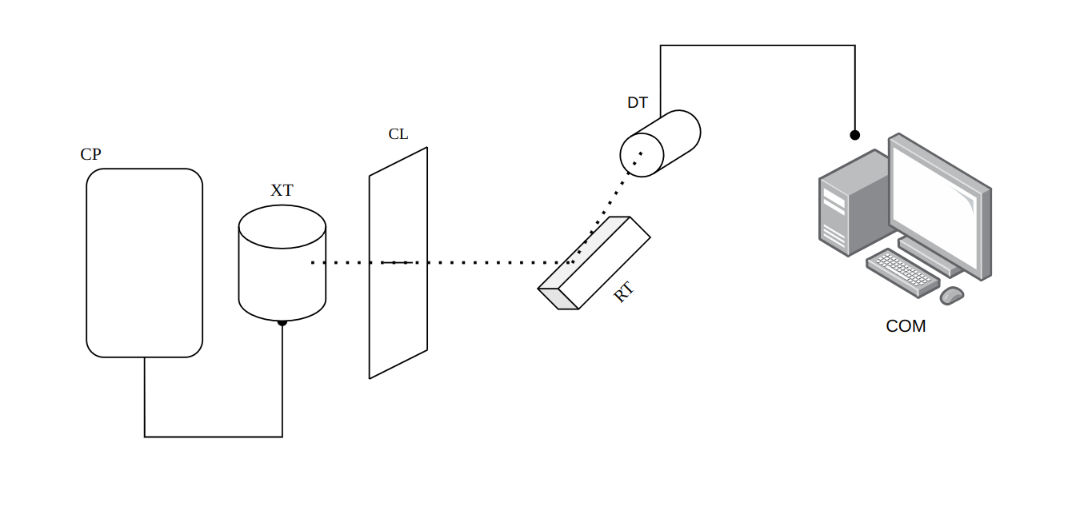
\includegraphics[width=0.8\linewidth]{3-xray/overleaf/images/xray_diagram.png}
    \caption{ \scriptsize{ Control Panel (CP), Copper X-ray Tube (XT), Collimation Wall (CL), Rotating Table (RT), Detector Tube (DT), Computer (COM).
    }}
    \label{fig:xray-diagram}
\end{figure}

\begin{multicols}{2}

\section*{Theory \& Procedure}
{
When stimulated, a copper anode emits two distinct characteristic X-rays: $K_\alpha$ and $K_\beta$. The $K_\alpha$ radiation, with a wavelength of 1.542 Å, occurs when an electron transitions from the $n=2$ shell to a vacant $n=1$ shell. In contrast, the $K_\beta$ radiation, with a wavelength of 1.392 Å, arises when an electron transitions from the $n=3$ shell to a vacant $n=1$ shell.

Given the extremely short wavelengths of X-rays, it is evident that a diffraction grating on the order of atomic dimensions is necessary to analyze the outgoing radiation effectively. To achieve this, we utilized \ce{LiF} and \ce{NaCl} crystals, along with a powdered LiF sample.

Crystalline materials have a periodic atomic structure that forms a lattice. In this lattice arrangement, when light is reflected from successive atomic planes, constructive interference occurs according to Bragg's Law, as described by Eq.\eqref{eq:1}. However, some of the X-ray's energy can continue to travel through the crystal.
\begin{equation}\label{eq:1}
    n\lambda = 2dsin\theta
\end{equation}
Where $d$ is the spacing between planes, $\theta$ is the angle the light is reflected back relative to the plane, n is the order of diffraction, and $\lambda$ is the wavelength.

Probing regular crystal structures with high-energy EM radiation allows us to study the near atomic scale structure of these materials, and record plane spacing in various orientations. The compounds \ce{LiF} and \ce{NaCl} both form face-centered cubic (FCC) crystal structures, which are more highly symmetric than many other crystal structures. FCC crystals allows for a specific set of allowed reflections, which leads to characteristic sequences of peak positions at well know Miller Indices. 

Using crystals in powdered form becomes more difficult to measure and interpret, because for non-powdered crystals the small-scale structure is in general uniform, but in powder form they appear non-uniform, making it difficult for reflected X-rays to successively exit the structure.

In crystal lattices the spacing between planes can be describe by the equation:
\begin{equation}\label{eq:2}
 d(hkl) = n\frac{a_0}{\sqrt{h^2+k^2+l^2}}
\end{equation}
where $a_0$ is the lattice constant and $n$ is an integer called the order of diffraction. Miller indices ($hkl$) classify the possible reflections in the X-ray diffraction pattern. For example, (\textbf{hkl}) = (\textbf{100}) comes from the planes parallel to the cube faces. And, (\textbf{hkl}) = (\textbf{110}) involves planes that cut through opposite edges of the cube.

To begin the experiment, we powered the Leybold Didactic (LD) X-ray apparatus. This apparatus holds 3 different sections: (1) the control panel, used to adjust experimental parameters, (2) the X-ray tube housing a copper anode, and (3) a Geiger-Müller detector positioned with the experimental sample. The apparatus also features lead glass shielding which controls the voltage switch (to the copper anode), allowing visibility while ensuring protection from X-ray exposure. Additionally, this whole device is connected to a computer where we can externally control starting parameters. 

For the measurements, we placed the desired sample on a rotating stage, which rotates at an angle of 2$\theta$ relative to the detector’s rotation $\theta$. Initial measurements were taken with the two crystal samples, which took approximately 15 minutes each. The powdered sample, due to its powdered nature, required around 3 hours for viable measurements. All measurements (for the whole-crystal) were recorded in 0.1\textdegree\ increments from 5\textdegree\ to 60\textdegree and timing increments were \SI{0.2}{\second}. For the powdered sample, the step duration was increased to \SI{14}{\second} due to the random (isotropic) orientation\footnote{Longer exposure time at each angular step is required to compensate for the reduced intensity of diffracted light.} of the many tiny crystals. Before each run, we reset the system to ensure the starting angle was calibrated at $\theta$ = 0. From here, we set our starting parameters, and started measuring. 
}
    
\section*{Analysis \& Results}
{
When analyzing the diffraction data for crystals you first notice that each peak occurs in pairs, with the less intense peak consistently corresponding to $K_\beta$. Each pair after should be understood as a increase in the order of diffraction $n$. By utilizing the measured angle $\theta$, the diffraction order, and the known wavelength $\lambda$, we can apply the Bragg condition to calculate the plane spacing $d$. From this, the lattice constant can be determined with $2d$. In this case, the Miller Indices can be found through a method of educated guesses. To do this we would enter specific even or odd combinations of hkl and using the specific combination we would attempt to find the lattice constant that matches a accepted value. We completed this step for every angle we measured in the powdered sample.

The results from the \ce{LiF} and \ce{NaCl} crystal are included in tables \ref{tab:LiF} and \ref{tab:NaCl}. The accepted lattice constant is 4.05 {\AA} and 5.68 {\AA} for \ce{LiF} and \ce{NaCl} respectively. Our measured lattice constant for \ce{NaCl}, 5.64 {\AA},is exactly the same as the accepted value, but for \ce{LiF} this measured value is not same. We suspect one of the systematic errors that may have caused this is that the sample may not have been as smooth as it needed to be. This could cause the x-rays to interact with the atoms in complicated ways at the surface. 

The results from the \ce{LiF} powder are shown in table \ref{tab:powder}. Peak 2 and 3 are reflections from the adhesive holding the powder together, this is the reason why very little data is given. The accepted lattice constant value of 4.05 {\AA} is not the same as any of the measured values or the mean value. We believe this is because when choosing a value for the angle of each peak, we were not as accurate as we needed to be. 
}


\end{multicols}

\section*{Summary}
{
In conclusion, this experiment demonstrated the principles of constructive X-ray diffraction on crystals and powdered crystalline samples. By using a copper anode to emit characteristic X-rays and a sophisticated detector, we observed distinct diffraction patterns. These patterns, governed by Bragg’s Law, allowed us to calculate key crystal properties such as the spacing between atomic planes and the lattice constant. These patterns also allowed us to gain a better understanding of how Miller Indices can describe the interaction X-rays have with different planes with varying orientations. In all, this experiment provided valuable insights into crystal structure and how X-rays scatter based on the arrangement and orientation of crystalline planes.
}

\begin{table*}[]
\centering
\begin{tabular}{c|c|c|c|c|c|c|c|c}
peak \# & angle ($^\circ$) & n & X-ray, $\lambda$ (m) & $d$ (m) & $a_0$ (m) & $\overline{a_0}$ (m) & $\overline{a_0}$ (\AA) & $\sigma_{\overline{a_0}}$ (m) \\ \hline
1 & 20 & 1 & $K_\beta$ & 2.14E-10 & 4.28E-10  & 3.12E-10 & 3.12 & 1.17E-10\\
2 & 22.5 & 1 & $K_\alpha$ & 1.97E-10 & 3.95E-10 \\
3 & 43.5 & 2 & $K_\beta$ & 9.67E-11	& 1.93E-10\\
4 & 49.6 & 2 & $K_\alpha$ & 1.16E-10 & 2.33E-10 \\   
\end{tabular}
\caption{Information for the \ce{LiF} crystal. $\overline{a_0}$ (m) \& $\overline{a_0}$ (\AA) are the average lattice constant in meters and Angstrom respectively. $\sigma_{\overline{a_0}}$ is the standard deviation in meters.  }
\label{tab:LiF}
\end{table*}

\begin{table*}[]
\centering
\begin{tabular}{c|c|c|c|c|c|c|c|c|c}
peak \# & angle ($^\circ$) & n & X-ray, $\lambda$ (m) & $d$ (m) & $a_0$ (m) & $\overline{a_0}$ (m) & $\overline{a_0}$ (\AA) & $\sigma_{\overline{a_0}}$ (m)  \\ \hline
1 & 14 & 1 & $K_\beta$ & 2.88E-10 & 5.75E-10 & 5.68E-10 & 5.68 & 7.51E-12 \\
2 & 15.6 & 1 & $K_\alpha$ & 2.80E-10 & 5.59E-10 \\
3 & 29 & 2 & $K_\beta$ & 2.87E-10 & 5.74E-10\\
4 & 32.8 & 2 & $K_\alpha$ & 2.83E-10 & 5.66E-10 \\  
\end{tabular}
\caption{Information for the \ce{NaCl} crystal. $\overline{a_0}$ (m) \& $\overline{a_0}$ (\AA) are the average lattice constant in meters and Angstrom respectively. $\sigma_{\overline{a_0}}$ is the standard deviation in meters. }
\label{tab:NaCl}
\end{table*}

\begin{table*}[]
\centering
\begin{tabular}{c|c|c|c|c|c|c|c|c|c|c}
peak \# & angle ($^\circ$) & h & k & l & X-ray type & $a_0$ & $\overline{a_0}$ (\AA) & $\sigma_{a_0}$ & $\sigma_{a_0}$/$\overline{a_0}$  \\ \hline
1 & 7 & 4  & 4  & 4  & alpha & 4.3831E-09  & 4.33E-10 & 3.15E-11 & 1.5098\\
2 & 8 & & &   & none & & & & \\
3 & 12 & & &   & none & & & & \\
4 & 16 & 0 & 0 & 2 & beta & 5.0501E-10 & & & \\
5 & 18 & 0 & 0 & 2 & beta & 4.5046E-10 & & & \\
6 & 22 & 0 & 0 & 2 & alpha & 4.1163E-10 & & & \\
7 & 28 & 0 & 2 & 2 & beta & 4.1932E-10 & & & \\
8 & 33 & 0 & 2 & 2 & alpha & 4.0040E-10 & & & \\
9 & 39 & 0 & 2 & 4 & alpha & 4.2440E-10 & & & \\
10 & 41 & 0 & 0 & 4 & beta & 4.2435E-10 & & & \\
11 & 49 & 0 & 2 & 4 & beta & 4.1242E-10 & & & \\
12 & 58 & 2 & 2 & 4 & alpha & 4.4539E-10 & & &        
\end{tabular}
\caption{Information for the \ce{LiF} crystalline powder. $\overline{a_0}$ (\AA) are the average lattice constant in Angstrom. $\sigma_{\overline{a_0}}$ is the standard deviation in meters.}
\label{tab:powder}
\end{table*}

\begin{figure}[tbh]
    \centering
    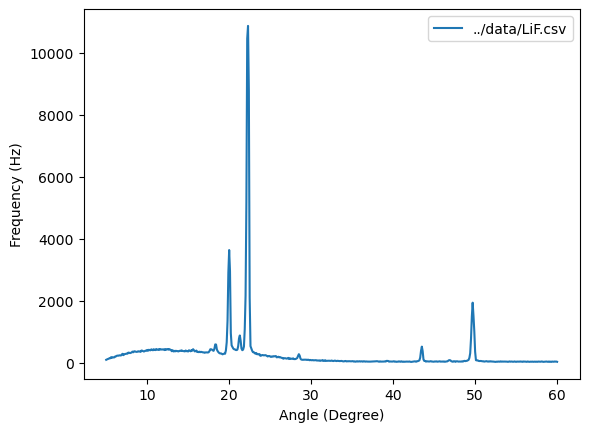
\includegraphics[width=0.8\linewidth]{3-xray/overleaf/images/LiF.png}
    \caption{ \scriptsize{ LiF Crystal Sample
    }}
    \label{fig:xray-diagram}
\end{figure}

\begin{figure}[tbh]
    \centering
    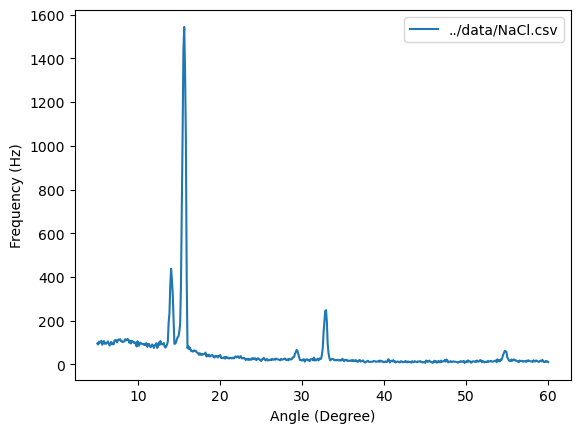
\includegraphics[width=0.8\linewidth]{3-xray/overleaf/images/NaCl.png}
    \caption{ \scriptsize{ NaCl Crystal Sample
    }}
    \label{fig:xray-diagram}
\end{figure}


\begin{figure}[tbh]
    \centering
    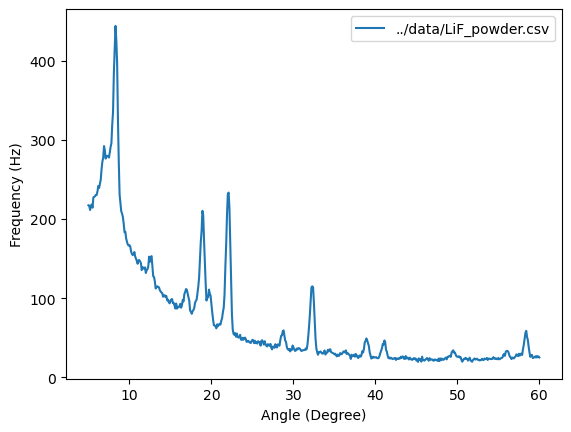
\includegraphics[width=0.8\linewidth]{3-xray/overleaf/images/LiD_powder.png}
    \caption{ \scriptsize{ LiF Powdered Crystal Sample
    }}
    \label{fig:xray-diagram}
\end{figure}

\end{document}